%\chapter{Results}


%This sections corresponds to the phases Data Mining and Interpretation of the Knowledge Discovery in Databases process. Here, we present two different analyses using the UDC and ABB datasets:
%\begin{enumerate}
	%\item Analysis of the impact of interruptions of work in the programmers' performance and activities
	%\item Identification and characterization of the programmers' activities at low level (activities within 5 minutes) and high level, covering working sessions.
%\end{enumerate}

%First, we present the analysis of the impact of interruptions in the following section.

\chapter{Interruptions of work and productivity}
In this chapter we present an analysis of the effects of interruptions of work in programmers' productivity, a phenomenon that has been previously investigated via field studies and to a wider spectrum of workers \cite{GM04, MGK08, CHW04, ABV12} instead of focusing on the population of programmers like this work. These studies agree that interruptions of work can be detrimental to the programmer performance, for every interruption demands a recovery or resumption time to restore the lost context.

To assess the impact of interruptions we use a set of metrics described in Chapter 3: edits per minute, selections per minute and edit ratio. We measure the effects on productivity using mainly the edit and selection events per minute as indicators. The edit ratio \cite{KM06} might be also a good indicator, under the assumption that a productive programmer will execute more editing activities than selection or navigation events. However, this is not always the case, given that depending on the role of the worker, selection events can be equivalent to the usage of a designing or reporting tool.

The results presented in this section correspond to a replica of a published paper \cite{SRV15} in the 22nd IEEE International Conference on Software Analysis, Evolution, and Reengineering. That paper included the same analyses described in the next three sections (4.1 to 4.3) but with a different dataset (Mylyn). During this work we improved some of the methodology and extended the results to include a detailed analysis of the Recovery Time (subsection 4.1.4). The extended version is now being submitted to the Journal of Software: Evolution and Process.

As we described in the Introduction, in this chapter we answer the following research questions:
\begin{itemize}
	\item RQ1: What is the relationship between the observed interruptions and the observed developer productivity?
	\item RQ2: Is the observed relationship more pronounced in the presence of prolonged interruptions?
	\item RQ3: What is the observed relationship in the vicinity of interruptions?
	\item RQ4: What events are more common during recovery time?
\end{itemize}



\section{Relationship between the number of interruptions and productivity}
As mentioned above, we use the metrics of edit, selection, and edit ratio as indicators of productivity. We first examine the number of edits and selections, and how their distribution varies in function of the number and type of interruptions.
%we assume that the productivity is in function of the number of edit and selection events that the programmer performs in a trace. 

%First, we analyzed the number of interruptions over the productivity. In this sense, 
We split the data in five groups: The first group contains all the sessions without interruptions (\textit{none}). For the others groups, we have considered four ranges of number of interruptions delimited by their quartiles, being 2, 4 and 7 the first, second and third quartile respectively.

\begin{figure}[!ht]
	\centering
	
		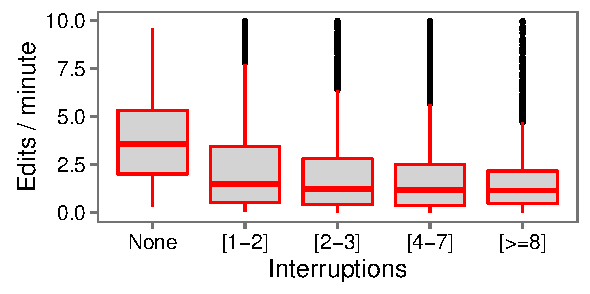
\includegraphics[width=0.6\linewidth,clip=, angle=0]{Figures/UDC_inte_emin}  
		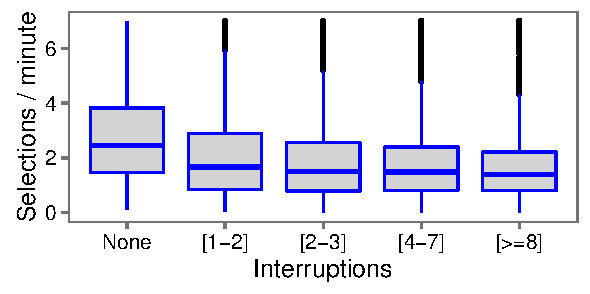
\includegraphics[width=0.6\linewidth,clip=, angle=0]{Figures/UDC_inte_smin}  
		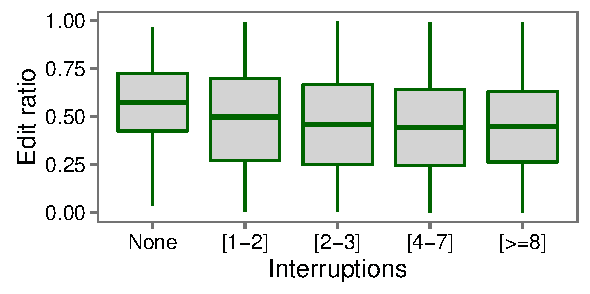
\includegraphics[width=0.6\linewidth,clip=, angle=0]{Figures/UDC_inte_eratio} 
	
	
	\label{fig:box_int_events}
	\caption{Boxplots showing the relation between the number of edits and selection events per minute, the edit ratio, and the number of interruptions. }
\end{figure}

We observe that when facing zero interruptions the editions and selections per minute are greater than in sessions with one or more interruptions, and as more interruptions occur the metrics gradually decrease. There is a big difference between sessions with no interruptions and at least one in the edits per minute metric.

As for the edit ratio, the median changes accordingly with the number of interruptions, decreasing when there are more and reaching the maximum when there are none. In addition, the size and form of the boxes indicate more variation in these results and the differences between groups is more subtle, judging by the small changes in the mean values.

Beyond visual inspection, we also quantify the statistical and the practical significance of these observations. First, all the differences observed are statistically significant with very low p-values (see Table~\ref{tbl:p_value_udc}) according to the Mann-Whitney U-test. This is not surprising, given the shape of the boxplots and the size of the samples. It is important to mention that the values from the effect size in the Table \ref{tbl:p_value_udc} are obtained by comparing the \textit{none} group with the rest of the groups.


More importantly, we used \textit{Cliff's delta} to measure the practical significance of these results in term of effect size % the effect size of the differences in means as standardized difference~
\cite{C94}. \textit{Cliff's delta thresholds} are defined as follows: negligible ($<0.147$), small  ($<0.33$), moderate ($<0.476$) and large effect otherwise. As shown in Table \ref{tbl:p_value_udc}, we note that the effect size of the interruptions over the number of edits per minute is overall moderate, being larger for edits per minute and small in the edit ratio. %Note that despite the differences in effect sizes, the differences are still significant and it is possible to reach the same conclusions.

\begin{table}[ht!]
	\small
	\caption{Effect size and significance of the relationship between number of editions per minute, selections per minute, edit ratio, and the number of interruptions on UDC data} 
	\label{tbl:p_value_udc}
	\centering
	\begin{tabular}{l | p{0.75cm} | p{1.2cm} | p{1.2cm} | p{1.2cm} |p{1.2cm}} 
		\hline
		& none & $\leq 2$ & $[3 - 4]$ & $[5 - 7]$ & $\geq 8$  \\  
		\hline
		\hline
		\multicolumn{6}{c}{\textbf{Edits}} \\
		\hline
		median & 3.58 & 1.5 & 1.23 & 1.15 & 1.18 \\
		\cline{2-6} 
		mean & 3.97 &	2.18 & 1.82 & 1.70 & 1.59 \\ 
		% \cline{3-6} 
		%t.test & $\hookrightarrow$& \multicolumn{4}{c}{$<$ 2.2e-16} \\
		\cline{3-6} 
		U-test (adjusted) & $\hookrightarrow$ & \multicolumn{4}{c}{$<$ 2.2e-16} \\
		\cline{3-6} 
		Cliff's delta & $\hookrightarrow$	& \textbf{0.42} & \textbf{0.53} & \textbf{0.57} & \textbf{0.63}    \\
		
		
		\hline
		\multicolumn{6}{c}{\textbf{Selections}} \\
		\hline 
		median & 2.54 & 1.66 & 1.5 & 1.5 & 1.4 \\
		\cline{2-6} 
		mean & 3.10 &	2.93 & 1.80 & 1.77 & 1.63  \\ 
		% \cline{3-6} 
		%t.test & $\hookrightarrow$& 6.258e-08 & 1.623e-12 & 4.87e-16 & $<$ 2.2e-16 \\
		\cline{3-6} 
		U-test (adjusted)& $\hookrightarrow$ & \multicolumn{4}{c}{$<$ 2.2e-16} \\
		\cline{3-6} 
		Cliff's delta & $\hookrightarrow$	& \textbf{0.29} & \textbf{0.38} & \textbf{0.39} & \textbf{0.49} \\  
		\hline
		
		\multicolumn{6}{c}{\textbf{Edit ratio}} \\
		\hline 
		median & 0.57 & 0.49 & 0.45 & 0.43 & 0.44 \\
		\cline{2-6} 
		mean & 0.68 & 0.56 & 0.55 & 0.54 & 0.57 \\ 
		\cline{3-6} 
		%    t.test & $\hookrightarrow$& 1.62E-13 & \multicolumn{3}{c}{$<$ 2.2e-16} \\
		\cline{3-6} 
		U-test (adjusted) &  $\hookrightarrow$& \multicolumn{4}{c}{$<$ 0.0001} \\
		\cline{3-6} 
		Cliff's delta & $\hookrightarrow$ & \textbf{0.19} & \textbf{0.24} & \textbf{0.28} & \textbf{0.26} \\ 
		\hline
		
	\end{tabular}
\end{table}

\section{Relationship between duration of interruptions and productivity}

In this section we analyze whether or not the duration of interruptions is a factor in the relationship between interruptions and developer productivity. Under the hypothesis that prolonged interruptions require more time to recover from, we built two groups of sessions based on the proportion of long interruptions. As we described previously we consider that a prolonged interruption has a duration of $\geq$ 12 minutes, a decision based on the literature \cite{GM04, KaptelininN07}. %Prolonged interruptions could be due to an extended interruption, such as a coffee break or a meeting.

For every session, we calculated the proportion of prolonged interruptions as the sum of interruptions with duration greater or equal than 12 minutes, divided by the total count of interruptions in that session. Then, we created 2 groups of sessions described as follows:

\begin{itemize}
	\item \textit{low}: the first group consists of sessions where the proportion of prolonged interruptions is $<$0.50; this includes sessions for which the proportion of long interruption is zero, that is, sessions with only short interruptions. They are the 38.7\% of all the sessions.
	\item \textit{high}: the second group consists of sessions where half or more of the interruptions are prolonged (proportion $\geq$0.50). This represents 60.1\% of the sessions.
\end{itemize} 

Following the conclusions on the last subsection, the number of interruptions has an impact on the metrics and should not be ignored. Furthermore, as the number of interruptions increases the difference between the groups minimizes.  %we believe that having   more distinctive groups instead of groups created by ranges is also valid.
Thus we want to compare the proportions of prolonged interruptions among sessions that have the \emph{same} number of interruptions. We hence split the \emph{low} and \emph{high} groups in subgroups of sessions which have the same number of interruptions. We consider groups of up to seven sessions, as larger groups tend to be smaller. We finally compare pairs of \emph{low} and \emph{high} groups that have the same number of interruptions, expecting higher productivity indicators in the \emph{low} groups.

The Figure \ref{fig:udc_rq2} shows the median of the metrics when grouping the sessions by the number of interruptions and the proportion of prolonged interruptions. According to our hypothesis, we expect sessions that have a low number of interruptions and a low proportion of prolonged interruptions to have higher rates of productivity, and the results mostly agree with this statement. First, we observe that when the number of interruptions increases the median of the metrics decrease until reaching a point (approximately between three and four interruptions) where the change is minimal and continues that way for the rest of the groups. Second, in the vast majority of groups the median value of the \emph{low} group is greater than the \emph{high} group.

\begin{figure}[!ht]
	\centering		
	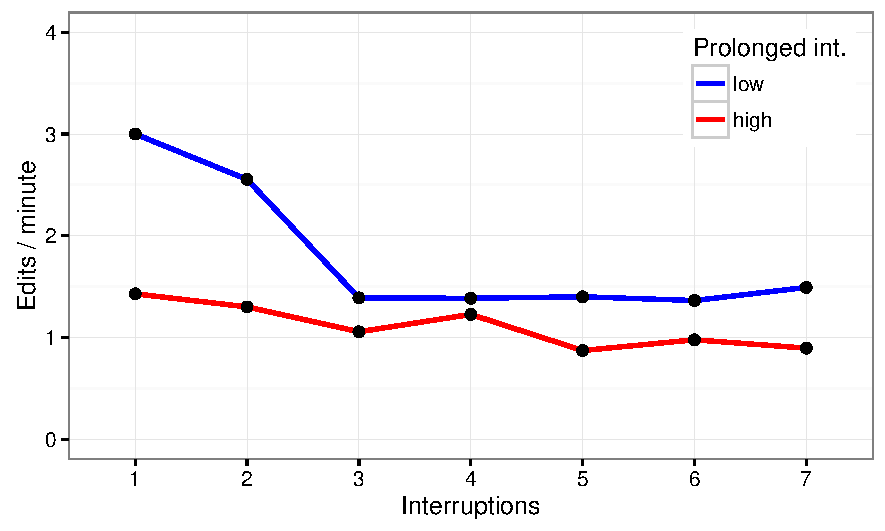
\includegraphics[width=0.5\textwidth]{Figures/UDC_rq2_emin}
	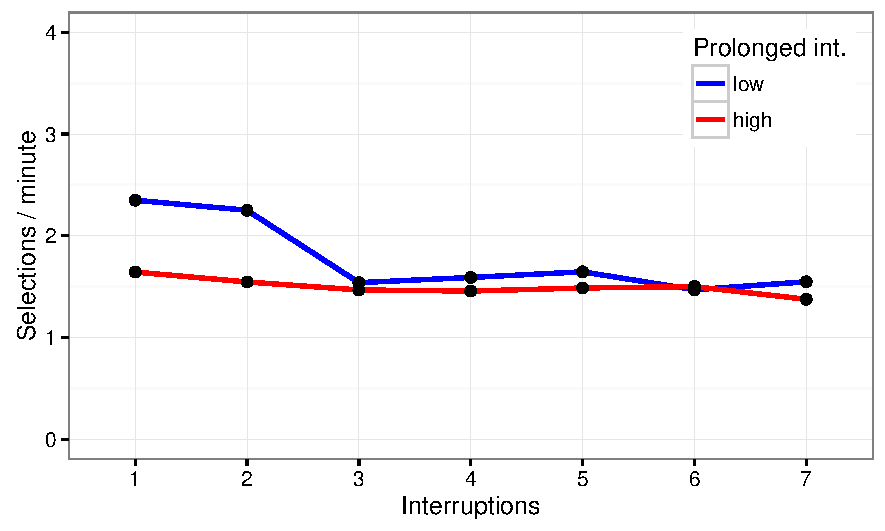
\includegraphics[width=0.5\textwidth]{Figures/UDC_rq2_smin}
	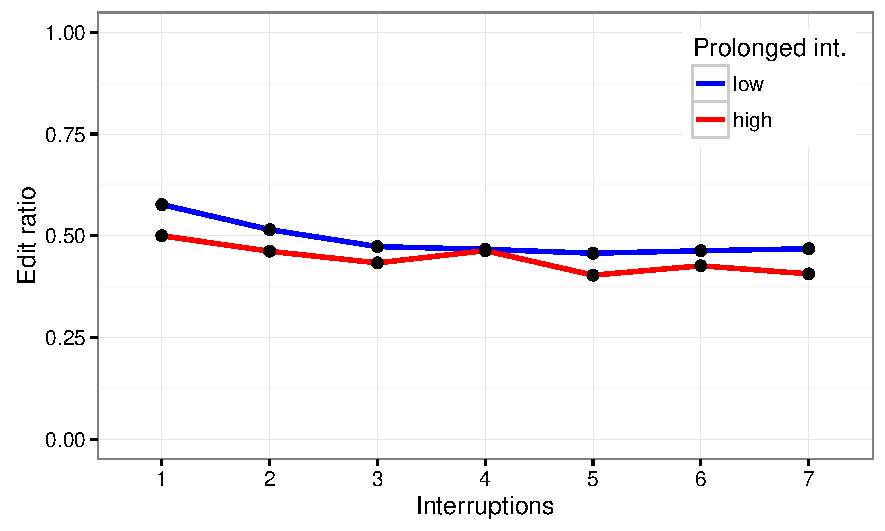
\includegraphics[width=0.5\textwidth]{Figures/UDC_rq2_eratio}

	\caption{Median values of edits and selection events per minute, and the edit ratio according to the number
		of interruptions and proportion of prolonged interruptions.}
		\label{fig:udc_rq2}
\end{figure}

When having a small number of interruptions (between 1 and 3) the difference between sessions with a low or high proportion of prolonged interruptions is very noticeable, and the group of sessions with a low proportion has higher median values. As the number of interruptions increases the differences get smaller, but we observe that the group of low proportion of prolonged interruptions usually shows higher values. This applies on the edits and selections per minute, and to a lesser extent to the edit ratio, where the changes between groups (both by number of interruptions and proportion) are comparatively smaller.

We tested the statistical significance of this results and show the results in the Table \ref{tbl:effect_size_dur_udc}. For every group according to the number of interruptions, we measured the effect between the low and high groups of sessions, with the Cliff's delta test and U-test. The groups with one or two interruptions have moderate size effects, in comparison with the other groups with more interruptions that have lower size effects; this matches our observations via visual inspection on a more defined difference between the low and high groups when having a small number of interruptions. Starting from (approximately) three interruptions, the distributions of the metrics are very similar.

\begin{table}[ht!]
	\small

	\caption{Effect size and statistical significance of the relationships between the groups of sessions by proportion of prolonged interruptions and the number of interruptions in UDC}
	\label{tbl:effect_size_dur_udc}
	\centering
	\begin{tabular}{l | p{1cm} | p{1cm} | p{1cm} | p{1cm} | p{1cm} | p{1cm} | p{1cm}} 
		\hline
		Group & 1 & 2 & 3 & 4 & 5 & 6 & 7  \\  
		\hline
		\hline
		\multicolumn{8}{c}{\textbf{Edits}} \\
		\hline
		U-test (adjusted) & 1.9e-20 & 4.0e-13 & 0.0011 & 0.027 & 7.2e-08 & 0.055 & 6.5e-06\\
		\hline
		Cliff's delta & \textbf{0.36} & \textbf{0.27} & \textbf{0.08} & \textbf{0.06} & \textbf{0.17} & \textbf{0.07} & \textbf{0.18} \\
		\hline
		
		\multicolumn{8}{c}{\textbf{Selections}} \\
		\hline 
		U-test (adjusted) & 2.9e-07 & 2.3e-11 & 0.32 & 0.12 & 0.0043 & 0.45 & 0.12 \\
		\hline
		Cliff's delta & \textbf{0.20} & \textbf{0.25} & \textbf{0.02} & \textbf{0.05} & \textbf{0.10} & \textbf{0.03} & \textbf{0.07} \\  
		\hline
		
		\multicolumn{8}{c}{\textbf{Edit ratio}} \\
		\hline 
		U-test (adjusted) & 3.5e-05 & 0.033 & 0.033 & 0.20 & 0.004 & 0.14 & 0.0059 \\
		\hline 
		Cliff's delta & \textbf{0.17} & \textbf{0.08} & \textbf{0.05} & \textbf{0.04} & \textbf{0.10} & \textbf{0.06} & \textbf{0.11}  \\
		\hline
		
	\end{tabular}
\end{table}

\section{Local relationships between interruptions and productivity}
The impact of work fragmentation could be more noticeable in the immediate minutes before and after an interruption occurs. On the one hand, after an interruption the programmer may carry out activities meant to recover the lost mental state, such as reading the code, debugging, reading notes and cues, and other resumption strategies \cite{PR11}. Depending on the interruption, the recovery could last about 15 minutes, according to the reports from field studies \cite{IH07, SBV98}. In the data from UDC, the sessions with duration of at least seven hours (commonly the working time of a software developer) have 11 interruptions in average; if we consider a recovery time of 15 minutes, the total time required to recover from the interruptions can be of two hours, which is about one quarter of the whole session.

%\RR{expand this paragraph, since a reviewer asks explicitely for that}
On the other hand, before the interruption there is a preparation phase when the interruption is imminent or expected, e.g. lunch time, a meeting and other scheduled events. In this phase the programmer might leave notes or comments in the code to recover the context after the interruption \cite{PD10}. Also, when the interruption happened because of a problem found by the programmer, he may try to solve it by reading the code, or using the debugger; after these resources are depleted, the next option is to ask to teammates or other external resources \cite{LVD06}, which generates an interruption of the work. The activities prior to the interruption are commonly associated with selection and navigation tasks, such as reading the code and navigating to another classes or files to try to find an answer to the problem. 

Having presented the global effect of the interruptions over the user productivity, we now focus on the local activity before and after interruptions. We take a maximum real time interval of 30 minutes around each detected interruption, obtaining a set of 97,984 time series. Then, we compute the median of all these subsequences as a generic local representation (Figure \ref{fig:udc_local_effect}). We also plot with dashed lines the median values of edits and selections per minute in the sessions with interruptions in order to give more context to the observed values.

\begin{figure}[!ht]
	\caption{Local effect of an interruption in the user activity.}
	\centering		
	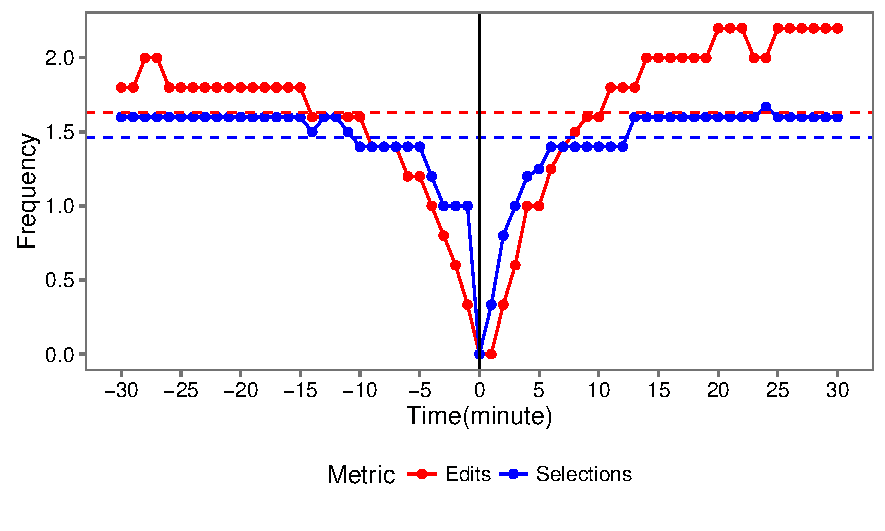
\includegraphics[width=0.8\textwidth]{Figures/UDC_local_effect}
	\label{fig:udc_local_effect}
\end{figure}

Below we describe some observations:
\begin{itemize}
	\item \textit{In the center,} we find the interruption point. There is clearly a negative effect on the time series, as the area before and after the interruption is the area with the lowest activity. The activity is well below the median activity of time series with interruptions, showing that the effect is indeed more pronounced near interruptions. 
	
	\item \textit{On the right,} the trend of the time series increases steadily. We hypothesize that the programmer is immersing again into the programming task, increasing progressively the activity as represented by the number of edits and selections. It reaches the median activity (in average) 6 to 12 minutes after the interruption. Then rises further than the session median, which is not surprising, as we expect higher than median activity further away from interruptions.
	
	%We called \textit{recuperation time} the first intersect point between edition and navigation. In this sense, the  average recuperation time of an interruption occurs in the minute 12. 
	\item \textit{On the left,} we observe that the number of events near the interruption also goes down well below the median value. This was more surprising at first to us. However we hypothesize that this might be because of two reasons: the programmer could have found a problem while coding, and at first would try to solve it by reading the code, switching out from the IDE, navigating the call stack and debugging, before going to ask another teammate (as documented e.g. by LaToza et al. \cite{LVD06}); this set of actions end up with an interruption and reduce the observed activity within the IDE. In the case when the interruption is imminent or expected, another possibility is that the programmer may make use of different suspension strategies such as writing physical notes, making a mental note or leaving a reminder cue on the code or window, as documented by Parnin and DeLine \cite{PD10}. These activities reduce the activity before the gap and they are seen in the interaction data mostly as selection events. The latest can be better visualized in Figure \ref{fig:udc_local_effect}, in which the UDC data has a significant decrease of edit events, being below the selection events approximately 10 minutes before the interruption.
\end{itemize}

\subsection{Patterns of Interruptions}
Given the overall activity pattern we noticed in the local analysis, we hypothesize that there are several kinds of interruptions, matching the scenarios observed in the literature: actual interruptions distracting the programmer from the task at hand, and switching tasks in case of being stuck in the current task.

We hence looked for patterns in the interruptions. After applying clustering techniques over all the subsequences, we always found the formation of three recurrent patterns that show different effects of the interruption: neutral, positive and negative. The clustering was performed with the  K-Mediods~\cite{AMP97} technique, the Silhouette metric~\cite{RP87} to interpret and evaluate the results, the Dynamic Time Warping~\cite{KE05} as distance measure, and feature extraction techniques to reduce the dimensionality.  For this reason, we classified empirically each interruption by its local effect. 

We did so by computing Cohen's $d$ on the quantity of edits before and after the interruption. To obtain a significant effect, we need the presence of activity both before and after the interruption. However, not all the interruptions meet this criteria: some are located close to the start or the end of a session, or too close to another interruption.  In total, 53\% of the interruptions had 30 minutes before and after the interruption and were selected for the analysis.  The remaining 47\% of the interruptions can not be used on this analysis due to the lack of time around them.


Table \ref{tbl:local_effect} shows the applied thresholds and the results. This local analysis shows that there are indeed three well-defined groups of interruptions, with the two largest of them having clear effects on the activity in the session. The 44\% of the interruptions are positive and the negative interruptions constitute the 44\%. The interruptions with a neutral pattern are the 12\%.


\begin{table}[ht!]
	\caption{Local effect of interruptions around 30 minutes. }
	\label{tbl:local_effect}
	\centering
	\begin{tabular}{m{6cm} | m{6cm}}
		\hline
		Effect & Pattern \\
		\hline
		\hline \\
		\textit{negative}: when the frequency of edit events decreases after the interruption (Cohen's $d < -0.2$)
		& 
		  \multicolumn{1}{m{3cm}}{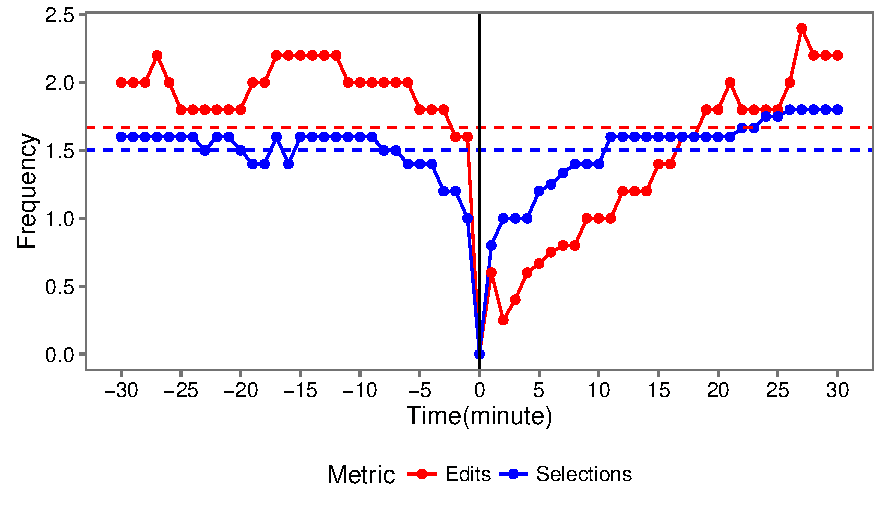
\includegraphics[scale=0.4]{Figures/UDC_local_effect_negative}} 
		      \\
		\textit{positive}: when the frequency of edit events increases after the interruption (Cohen's $d > 0.2$)
		& \multicolumn{1}{m{3cm}}{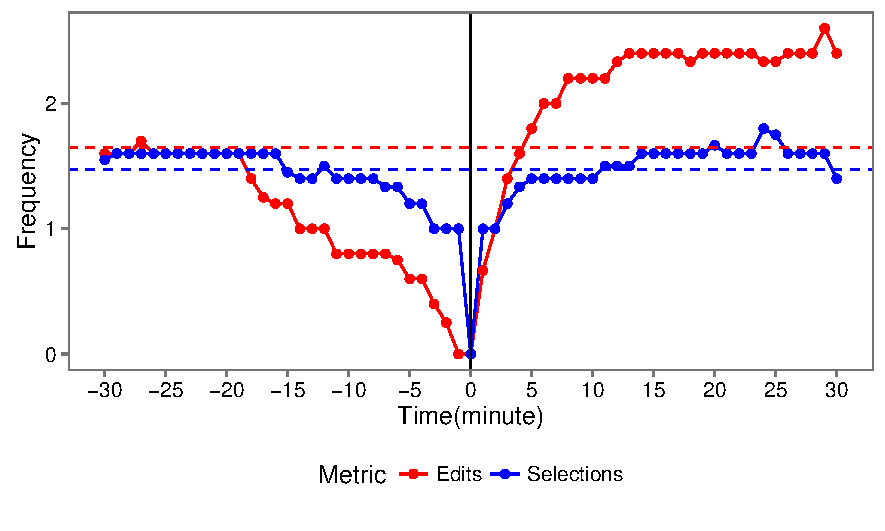
\includegraphics[scale=0.4]{Figures/UDC_local_effect_positive}} 
		\\
		\textit{neutral}: when there is no well defined effect before or after the interruption ($abs(d) <= 0.2$)
		& \multicolumn{1}{m{3cm}}{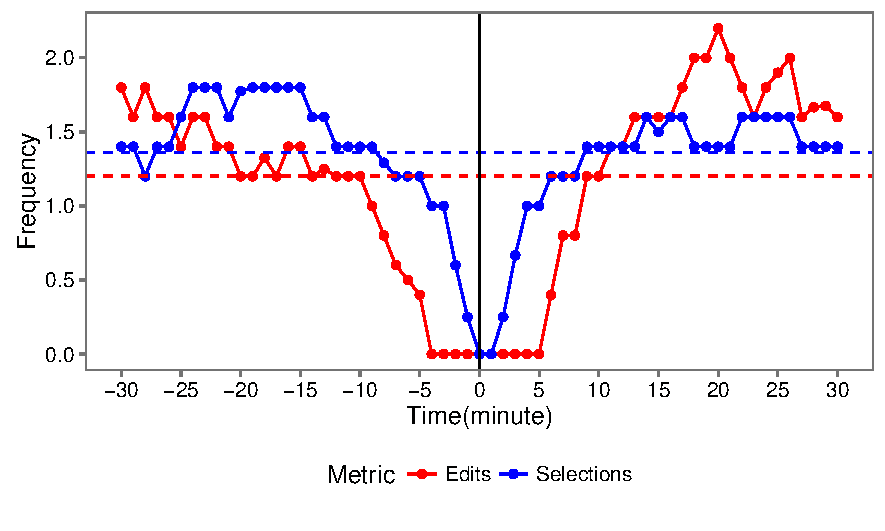
\includegraphics[scale=0.4]{Figures/UDC_local_effect_neutral}} 
		\\
	\end{tabular}
\end{table}

The results in UDC indicate that after a positive interruption, both metrics tend to increase at a high rhythm until reaching the global average value. The edits per minute recover quickly (approximately 5 minutes after the interruption), but the selections per minute take a little longer to reach the global average, and this metric tend to be below the average for an extended period. It is important to notice that before the interruption happens the editions per minute metric is below the average for approximately 16 minutes prior to the interruption.

In contrast, when facing the effects of a negative interruption the metrics take longer to reach the median. Contrary to when facing a positive interruption, the editions per minute metric is below the selections per minute, and the former takes longer than the latter to reach the average value. Also, the editions per minute metric is above the average for the 30 minutes before the interruption. 

In general, the effect of positive and negative interruptions seems to be reversed. The editions per minute describe better the effect and the selections do not show a major change. There is not a clear pattern during a neutral interruption.

\section{Recovery Time after an interruption}

In the last section we saw different patterns of activity around positive and negative interruptions. In particular, we observed that the edits per minute were higher after a positive interruption and the contrary after a negative interruption.

The presence of this pattern and the important difference observed in Figure \ref{fig:udc_local_effect} led us to investigate the effect more closely. To this aim, we did an exploratory study of the activities performed by programmers during the recovery time of an interruption. This is possible due to the high variety of events present in the UDC dataset, which can tell us a lot more about the type of activities that developers do.

The goal of the exploratory study was to better understand whether the activity taken after an interruption were indicative of different types of behavior for each type of interruption (positive or negative), and also whether these different kinds of activities supported our earlier hypotheses explaining why the two patterns of interruptions were present. Assuming that different commands represented different types of activity, the hypothesis was that the frequency of a given activity (as represented by the commands used to carry it) would vary between the different types of sessions.

A first challenge that we encountered was that the high number of different commands made it hard to infer broader trends. Hence, we used the detailed classification described in Chapter 3. With these categories we continue with describing the hypotheses we made earlier when we observed the positive and negative patterns, namely that:

\begin{enumerate}
	\item \emph{Negative} interruptions (having higher overall activity before the interruptions rather than after it) could be indicative of actual interruptions. That is, a programmer is interrupted in his normal course of work, and needs to rebuild his or her mental context after the interruption, performing additional program comprehension before resuming programming.
	\item On the other hand, \emph{Positive} interruptions (with higher activity after the interruption) could be indicative of information-seeking behavior. Programmers, noticing that they are encountering a problem that they are not able to fix on their own may look for outside help (asking an expert, querying a question and answer site such as Stack Overflow, etc), and once a solution is found, resume their work in the IDE in a much more productive manner.
	%\item \RR{What about debugging sessions?}
	\end{enumerate}

We would then expect that certain types of interruptions would feature some events more frequently than other ones. For instance, after a negative interruption, we would expect more program navigation events (indicative of program comprehension), while after a positive interruption, we would expect more programming activity since the problem that the programmer encountered was solved. In short, we expect that for some categories of events, there will be differences between the types of events. We put this hypothesis to the test by calculating the frequency of categories of events after positive and negative interruptions, and also compared it with the overall frequencies of the events. We describe how we computed these frequencies in the following.

First, we noticed that while some events are used by all users, other events are used heavily by a minority of users and not by others; this matches the observation of Murphy-Hill et al. \cite{MPB12} that many development tools are underused. For example, the event \textit{copyLineDown} is more frequent than the \textit{rename} event, but the former is only used by 2.4\% of the users and the latest by 25.2\% of them. As such, we calculated the frequency of event taking into account how commonly used they were.

We calculated the weighted average of every event based on the frequency of execution during the first phase of recovery time after a positive or negative interruption, and the percentage of users that make use of that event (so that events that are used by very few users do not distort the results). The weighted average was calculated as: $$\bar{x} = \frac{\sum_{i=1}^{n}w_ix_i}{\sum_{i=1}^{n}w_i} $$where $x_i$ is the frequency of execution of the event $i$ and $w_i$ is the percentage of users that uses the event. This balances the average of execution for events used by a small number of users. 

To get a baseline, the same frequency calculation was made for the entire dataset, without distinction of the location of events in the session. We then compared the weighted average changes to have evidence of what kind of events are more often executed after a positive or a negative interruption. The Table \ref{tbl:stats_events} shows the results, and is explained below.

\begin{table}[ht!]
	\small
	\caption{Weighted frequency of execution after positive or negative interruptions. }
	\label{tbl:stats_events}
	\centering
	\begin{tabular}{p{3cm}|p{2cm}|p{2cm}|p{2cm}} 
		\hline
		Category & Positive & Negative & All \\  
		\hline 
		\hline
		\multicolumn{4}{c}{\textit{Categories that are more frequent after a positive interruption}} \\
		\hline 
		Edit-Text &  \textbf{34.75} & 22.35 & 26.62 \\
		File &  \textbf{10.56} & 9.53 & 10.01\\
		Refactoring & \textbf{1.29} & 0.84 & 1.01 \\
		\hline 
		\multicolumn{4}{c}{\textit{Categories that are more frequent after a negative interruption}} \\
		\hline 
		High-Nav & 7.84 & \textbf{10.14} & 8.74  \\
		Debug & 3.08 & \textbf{7.81} & 6.35  \\
		Search & 1.81 & \textbf{2.43} & 1.84 \\
		Clean-Build & 0.42 & \textbf{0.62} & 0.56  \\
		Tools & 0.40 & \textbf{0.59} & 0.50 \\
		\hline 
		\multicolumn{4}{c}{\textit{Categories that are less frequent during the recovery time}} \\
		\hline 
		Text-Nav & 14.20 & 12.89 & \textbf{16.13} \\
		Control & 1.21 & 1.75 & \textbf{1.82} \\
		\hline
	\end{tabular}
\end{table}

After positive interruptions the events belonging to the Edit-Text, File and Refactoring categories are more frequent than in the average. In addition, these categories of events are less frequent than the average after a negative interruptions. Of these three, Edit-Text and Refactoring have the largest differences between positive and negative interruptions. This three categories are much more clearly associated with edition activities than program comprehension, and thus fit the previous hypothesis.

After a negative interruption, Debug, High-Nav, Search and Clean-Build categories are all more common than average. The categories of Debug, Search, and High-Nav are clearly associated with program comprehension rather than program edition. The Clean-Build category is not strongly associated with program comprehension, but it is however associated with debugging activities. 

Finally, the Text-Nav and Control categories are less common in both positive and negative interruptions than in the average. We were somewhat surprised that Text-Nav was less common in positive interruptions than the average, as we expected it to be associated with program edition behavior. We note that it is however more frequent in positive interruptions rather than negative interruptions. Additional exploration is necessary to understand the behavior of the Control category.

Summing up, we can conclude that edition-related activities are indeed more frequent after a positive interruption, while comprehension-related activities are more frequent after a negative interruption.  These categories of events agree with our previous hypothesis that positive interruptions are related to information seeking behavior: programmers would interrupt their IDE activities when encountering a roadblock, find the information elsewhere (from the Internet, an expert, etc), and return to the IDE with an increased productivity. This also agrees with the literature \cite{PR11, LVD06}. The categories common after negative interruptions also agree with our hypothesis that negative interruptions are related to actual task switches where context needs to be rebuilt afterwards, an activity that involves program comprehension \cite{MMLK14, PR12}. %\RR{refs here}.

Of course, this exploratory study does not allow us to confirm these hypotheses. However, the evidence we have discovered so far does not disprove them, and rather goes in the direction of our hypotheses, which means that our confidence in these hypotheses is higher as a consequence.

\chapter{Activities and Working Patterns}
There are numerous ways to identify the kind of activities and working patterns performed by programmers, such as through observational studies \cite{GM04}, surveys \cite{PR11}, usage data \cite{MPB12} and activity logs \cite{CLQ15}, being the first the one that provides richer information. Usage and activity data has been widely used to analyze activity patterns from programmers as part of the Mining Software Repositories research area, but the kind of activities that can be assessed depends on the available data. In this case, our approach to identifying activities and working patterns is by analyzing the execution frequency of certain events.

Recalling from the Introduction, these are the research questions we take on this chapter:
\begin{itemize}
	\item RQ5: What kind of activities can be identified with usage data?
	\item RQ6: What working patterns during a session are commonly performed by developers?
\end{itemize}

\section{Identifying activities}
In the literature we can find evidence about the kind of activities performed by programmers, mostly from observational studies and usage data \cite{LVD06, GM04, MMLK14, MKF06}. We could have defined a set of activities based on the conclusions from these resources, but how can we assure that the same activities are present in our data? Do we have enough data to identify those activities? Is the same kind of activities identifiable in both datasets? These are some of the problems in establishing a set of activities based on related work. \begin{changedforreviewerlong}
To avoid them, we used clustering techniques to discover the activities: they will find groups of similar chunks according to their attributes and each of these group will represent a different activity. \end{changedforreviewerlong} This way we can find a set of common activities according to the data and the thresholds to differentiate between them.

\begin{changedforreviewerlong}

During the Transformation phase we obtained a set of sessions and decomposed each into chunks of smaller size. According to the literature \cite{GM04}, in average, a task can last for at least 3 minutes. By creating chunks of 3 to 5 minutes we try to model the minimum activity unit; some activities might be of that size but others will require several chunks to cover them. Also, taking small time frames allowed us to observe activities that require just a few events.

\end{changedforreviewerlong}

Every one of these chunks has the proportion of execution of events by detailed type. So, the observations that were clustered are chunks and the attributes are the proportions. This means we have two datasets with 43,769 (UDC) and 23,624 (ABB) observations with 11 numerical attributes each. That is, the attributes represent the proportion of execution of events of the type Edit-Text, Text-Nav, High-Nav, Debug, Search, Refactoring, Testing, Control, Clean-Build, File and Tools.

\subsection{Preliminary studies}
As we do not know the number of activities we need an algorithm that chooses the number of clusters based on the data provided, such as Mean Shift, Affinity Propagation and DBSCAN. We need an implementation that allows us to explore the values for each of the axis (attributes) of the found clusters, so we only considered Mean Shift and Affinity Propagation.

We explored different models before arriving to the final approach; those models were compared using the Silhouette Coefficient and chose the one that offer the best values. The Silhouette Coefficient \cite{R87} is a value per data point where high values are obtained from well defined clusters. It is composed of two scores: $a$ representing the mean distance between a sample and all other points of the same cluster, and $b$ the mean distance between a sample and all other points in the next nearest cluster. So, the Silhouette Coefficient $s$ of a point is obtained as:

$$s = \frac{b-a}{max(a,b)}$$

This coefficient evaluates the compactness (how close are objects within the same cluster) and separation (how well-separated is a cluster from other clusters). It is a value between -1 and 1; a value of 1 indicates that the point is correctly clustered and a -1 indicates that it is probably contained in the wrong cluster. Values around 0 means the observation lies between two clusters. We use the average Silhouette Coefficient (also known as the Silhouette width) to compare between models and to conclude if there is an actual structure in the data. The Table \ref{tbl:silhouette} contains an interpretation for the Silhouette Coefficient.

\begin{table}
	\caption{Interpretation of the Silhouette Coefficient.}
	\label{tbl:silhouette}
	\centering
	\begin{tabular}{c | c }
		\hline 
		\emph{Range of values} & \emph{Meaning}\\  
		\hline 
		\hline
		0.71 - 1.0 & A strong structure has been found\\
		\hline
		0.51 - 0.70 & A reasonable structure has been found\\
		\hline
		0.26 - 0.50 & The structure is weak and could be artificial.  \\
		\hline	
		$\le$ 0.25 & No substantial structure has been found \\
		\hline
		
	\end{tabular}
\end{table}


In other topics, Mean Shift \cite{CM02} discovers centers based on the density of samples of a set of regions whose size relies on the parameter $bandwidth$. It updates possible centroids so they are mean of the samples within a given region. Afterwards, the centers that are near-duplicate are summarized and then it presents the final set of centers. After some initial experiments, the results with this algorithm tend to contain a small number of clusters; it finds very common activities but ignores some rare that are absorbed by more general clusters. %This is reflected in low average values of the distance within clusters, which is translated into bad Silhouette Coefficients, a metric described later.

Affinity Propagation \cite{FD07} creates clusters by sending messages between all the data points; this message contains a value indicating how suitable is a point to be an exemplar, and the accumulated values of the messages are used to make a decision. This is performed until high-quality exemplars are found and corresponds to a cluster. We observed after some experiments that this algorithm tends to create a high number of clusters, providing all kinds of activities but some of them at many levels; this means that several clusters cover one activity (e.g. Programming) but at different levels of intensity (e.g. high usage of Programming and low usage of Programming). This can be seen as the contrary effect of the Mean Shift results and with bad Silhouette averages. The main drawback of this algorithm is the high time-complexity of the order $O(n^2t)$, where $n$ is the number of samples and $t$ the number of iterations.

\subsection{Approach to the final model}
The issues of implementing only one clustering technique were solved with the following approach:

\begin{enumerate}
	\item First, cluster the observations with K-means into $k$ clusters. The parameter $k$ should be considerably big.
	\item Then cluster the resulting centroids with Mean Shift selecting a bandwidth $b$.
	\item Finally, label the observations according to the centroids of the second model.
\end{enumerate}

By clustering first with K-means we approximate the number of clusters with an algorithm with lower time-space complexity. The value for $k$ should be many times greater than the actual number of centers we expect to see. With this we try to cover all the probable activities, common and rare. The resulting clusters will be separated enough (and without much elements in between) so that they will not be summarized into one or two when applying the second clustering algorithm.

We still do not know what kind of activities are present in the data, so we need an algorithm that helps us discover them. For that, we cluster the centroids obtained from K-means with Mean Shift choosing a bandwidth $b$. To set the values for $k$ and $b$ we selected those that maximize the average Silhouette width. For ABB the parameters that maximize the metric are $k=3000$ and $b=0.41$. And for UDC the parameters should be $k=2500$ and $b=0.33$. With this approach we not only obtained acceptable clusters in terms of the activities they represent (seven clusters for ABB and nine for UDC), but also got models with good Silhouette width (0.55 for ABB and 0.38 for ABB). Mean Shift by itself also provides models with acceptable average Silhouette width at the expense of reducing the number of clusters, in some cases resulting in only two.

\subsection{Labeling the centers}
After we have the centers from Mean Shift, the next step is to add a label to each of them considering the values of the attributes. We took advantage that a high value for one of the attributes indicates that the activities of that center have heavy use of that event. Every center has a group of attributes with higher values than the rest; for example, a center labeled as Debugging has a value of 0.8 for the Debug attribute, and a value close to 0 for the rest, and a center labeled as Programming has higher values for the Edit-Text and Text-Nav attributes. The task involves manual work and the interpretation from the authors of what activity a cluster is modeling, so this could be a threat to the validity of the results. 

The assigned label represents the activity that a center models and several centers could represent the same activity. The Table \ref{tbl:activities} shows the resulting activities for ABB and UDC.

\begin{table}
	\caption{Activities found via clustering for UDC (left) and ABB (right).}
	\label{tbl:activities}
	\centering
	\begin{tabular}{c | c }
		\hline 
		\emph{Activity} & \emph{\% of chunks}\\  
		\hline 
		\hline
		Programming & 43.41 \% \\
		\hline
		Navigation & 38.05\%\\
		\hline
		Debugging & 6.69 \% \\
		\hline	
		Tool-usage & 4.27\% \\
		\hline
		File-mgmt & 3.80 \% \\
		\hline 		
		Version & 2.88 \%\\
		\hline
		Search & 1.16 \% \\
		\hline
		Refactoring & 0.47 \% \\
		\hline
		
	\end{tabular}
	\quad
	\begin{tabular}{c | c }
		\hline 
		\emph{Activity} & \emph{\% of chunks}\\  
		\hline 
		\hline 
		Debugging & 44.45 \% \\
		\hline
		Programming & 34.67 \% \\
		\hline
		Navigation & 17.20\%\\
		\hline
		Version & 2.77 \%\\
		\hline
		Tool-usage & 0.54 \% \\
		\hline
		Testing & 0.37	 \% \\
		\hline
	\end{tabular}
\end{table}

\section{Comparing activities between datasets}

Five activities (Programming, Navigation, Versioning, Debugging and Tool-usage) are present in both datasets and the rest are unique. We can see more variety of activities in the UDC dataset, which we attribute to the different types of programmers and to the sort of events that can be captured from the IDEs.

There are some interesting differences. First, the Programming activity is common in both cases with a high percentage of activities (43.41\% in UDC and 34.67\% in ABB), and surprisingly Debugging is only common in ABB (44.45\%), falling to the third place in UDC with only 6.69\%. Both datasets contain a very similar amount of events classified as Debug, that is 68 for UDC and 76 for ABB. The common events of control such as start debugging, step over and step into are present in both datasets, but the difference lies is in the 8 extra events available in ABB. 

The ABB programmers, which are Visual Studio users, make heavy use of the Locals Window of Visual Studio that allows them to explore the state of the objects when debugging and change around processes and threads. Eclipse has a similar functionality in the Debug Perspective and captures an event when the programmer use it, but it does not support exploring different instances in the same fashion as Visual Studio. On top of that, in the ABB data the most common events of the type Debug are in fact those that allow to change the current process or thread. This could be the main cause for the differences of Debugging activities between datasets.

Another difference is that Navigation and Tool-usage activities have more incidence in the UDC data. First, in respect to Navigation, UDC users seems to perform more navigation around tabs and search for classes from the Package Explorer of Eclipse, also noted by Murphy et al. \cite{MKF06}. In the other hand, ABB users commonly perform navigation around the hierarchy of classes by calling to definitions. The kind of navigation performed by UDC users is translated into much more navigation events of high level and it is referred as unstructured navigation \cite{AFQ15}.

The amount of Tool-usage activities is related to the variety of programmers in the UDC data in contrast with ABB. In the former there are a group of users that are Web developers and execute events involving PHP, JavaServer Faces, HTML and CSS. To a lesser extent, there are also SQL and J2EE (Java Enteprise Edition) developers. In ABB the small amount of Tool-usage activities is mostly related to the design of classes and architecture of the system in development, and also to connections to SQL databases. From this, we can infer that the programmers in ABB have mostly \emph{back-end} roles and probably maintain an existing system that is supported by a multithreading paradigm, judging by our observations on the Debugging activities. However, we are unable to ascertain these assumptions.

\begin{changedforreviewerlong}
We observed that all of theses activities has been identified and characterized before during observational studies. For example, from the categories found by Singel et al. \cite{SLV10}, we can match our findings with the debug, edit, management, search and testing categories. And from LaToza et al. \cite{LVD06} research we found editing, writing, unit testing and possibly non code. The Tool-usage activity we found is harder to relate to a category from the literature, for it can represent a wide range of tools used in a variety of activities, such as designing, configuration and in-house tools, from the Singel et al. categorization. Program comprehension (or understanding) is a common activity that is difficult to identify by itself in usage data given that it involves reading, debugging and navigating. We found the last two activities but we lack information to identify when they are executed due to program comprehension. So, answering the research question RQ5, we can identify at least 5 types of activities in usage data and the amount depends on the kind of information in the dataset and the type of events that can be captured from the IDE. From our two datasets we found Programming, Navigation, Debugging, Tool-usage and Versioning in both. The other activities File-management, Search, Refactoring and Testing depends on the dataset.
\end{changedforreviewerlong}

\section{Identifying patterns of sessions}
During a working session, a programmer could go throughout several states or perform multiple activities. It might be possible to understand better these activities by using the information of the clusters we obtained in the previous subsection. 

In this section we look for patterns of sets of activities (sessions) that might be common among programmers. Due to the nature of the data we expect to see more common patterns in the ABB data and more variety in the UDC data, for more kind of programmers are present in the latter.

Once we had the chunks clustered and labeled, we divided the chunks of each session into three groups of equal size representing the beginning, middle and end. We selected 4 activities that are present in both datasets (Programming, Navigation, Debugging and Version), to facilitate the comparison, and calculated the proportion of each at every phase. After that, every observation (session) had 12 attributes and proceeded to cluster them using the Affinity Propagation technique; this time we want to see all the possible clusters without limiting to a low number as when clustering with chunks and this algorithm can offer us a variety of patterns from which we analyzed the most common.

We found 47 clusters in ABB and 98 in UDC, but we only work with the 5 more populated. The Figure \ref{ABB_phases} shows the results for ABB and the Figure \ref{ABB_phases} for UDC. The Types (A to E) are ordered from the most to the less populated. This selection covers 35\% of the sessions in ABB and 39\% in UDC. 

\begin{figure}[!ht]
	
	\centering
	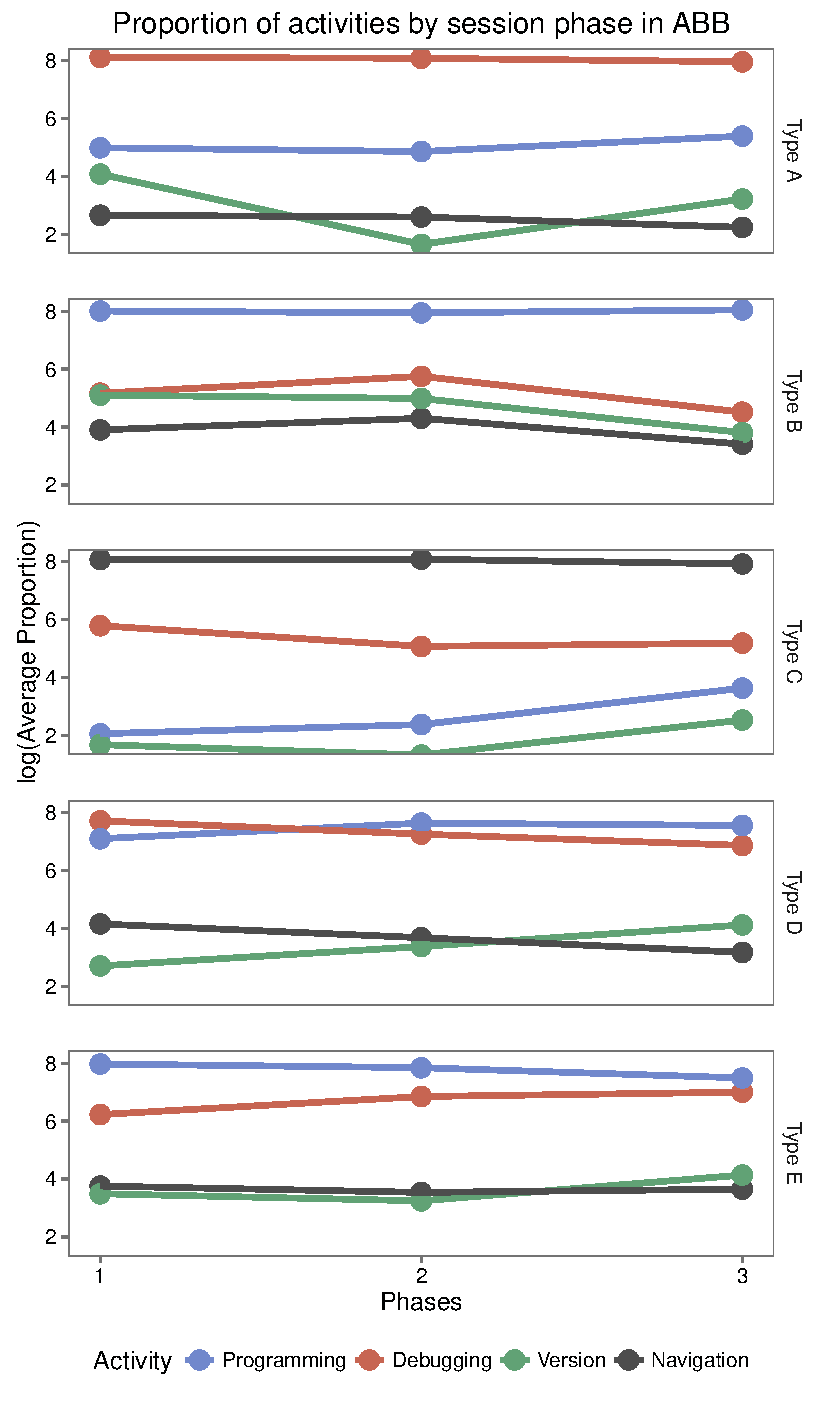
\includegraphics[width=0.6\textwidth]{Figures/ABB_phases_log}
	
	\caption{Most common patterns of activities in ABB.}
	\label{ABB_phases}
\end{figure}

\section{Comparison of working session patterns}


For the sessions from ABB in the Figure \ref{ABB_phases} we have the following observations:
\begin{itemize}
	\item The most common pattern (Type A) involves mostly Debugging activities throughout the session and it is followed by Type B, where the most common activity is programming throughout the session as well; it could be an effect of the two more frequent activities.
	
	\item The pattern described by the Type C is mostly composed of Navigation activities followed by Debugging. This can be related to program comprehension sessions \cite{MMLK14} or bug fixing due to the low amount of Programming.
	
	\item Types D and E have a fair amount for all the activities throughout the sessions and do not show notorious changes. Also, both Debugging and Programming are executed frequently, whence we relate these two patterns to multitasking sessions \cite{SLV10}.
	
	\item Versioning tasks are common during all the session when Programming is also a common. However it is only common at the beginning or ending of the session when the Programming tasks are low. It could be that during Programming activities the user reaches more checkpoints that should be committed. 
\end{itemize}

\begin{figure}[!ht]
	
	\centering
	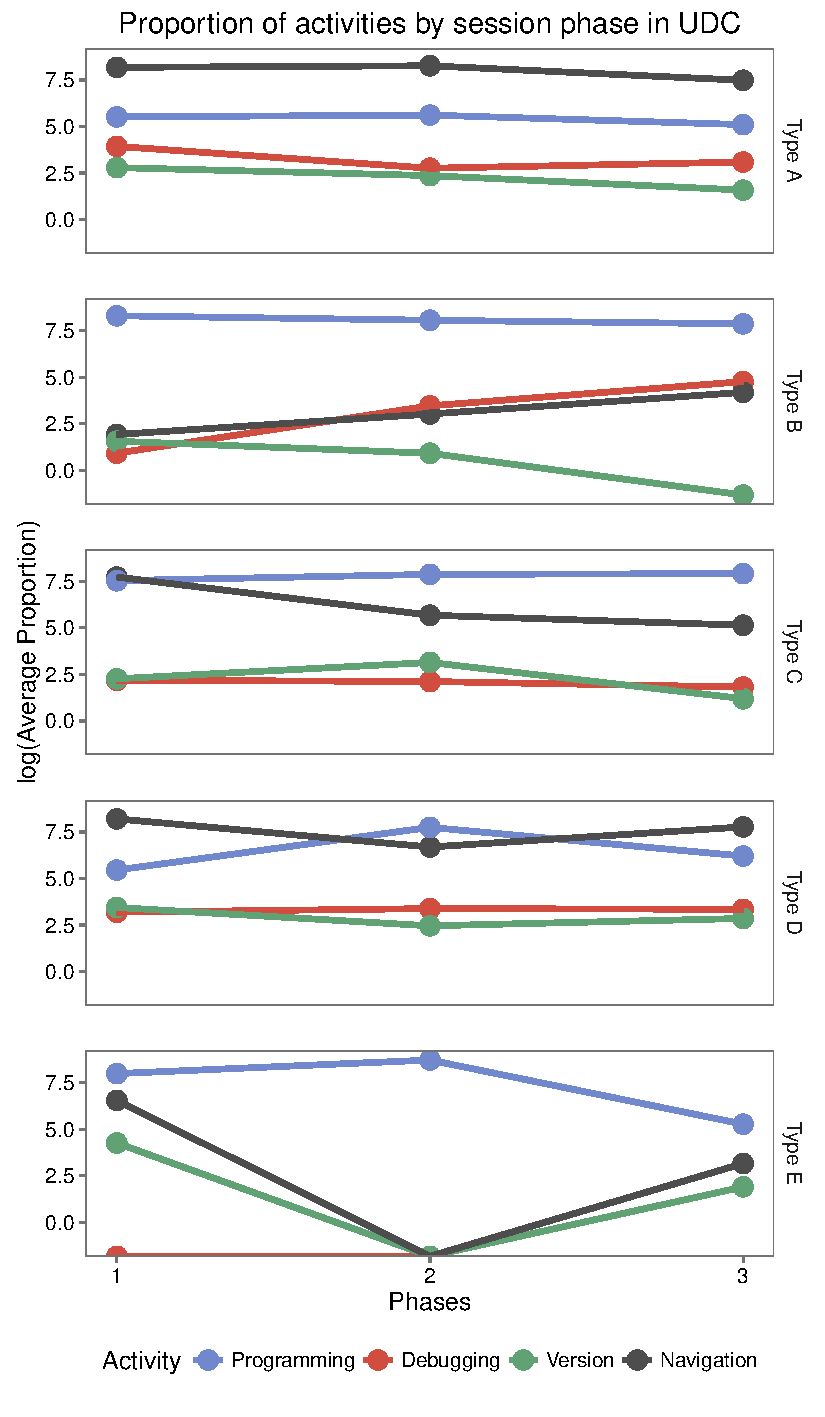
\includegraphics[width=0.6\textwidth]{Figures/UDC_phases_log}
	%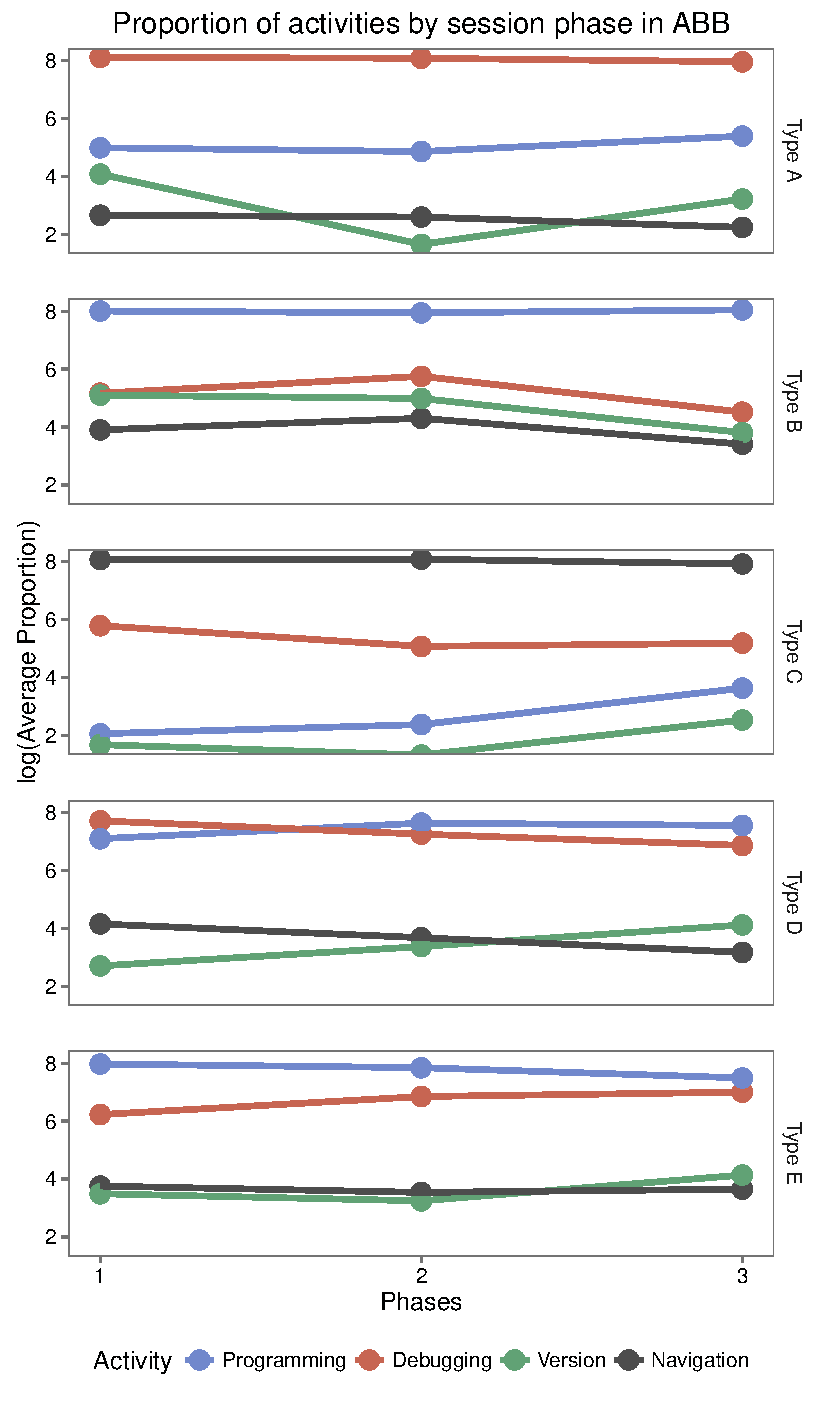
\includegraphics[width=0.49\textwidth]{Figures/ABB_phases_log}
	
	\caption{Most common patterns of activities in UDC.}
	\label{UDC_phases}
\end{figure}

For the sessions from UDC in the Figure \ref{UDC_phases} we have the following observations:
\begin{itemize}
	\item We relate Types A, C and D to multitasking sessions. The activities do not suffer sudden changes on any of the three phases.
	
	\item Type B keeps a steady amount of Programming throughout the session and there is a gradual increase of Debugging and Navigation until reaching a peak at the end. This is an interesting pattern that could be related to an increase of testing and proof of concept towards the end of the session.
	
	\item The sessions with a pattern of the Type E lacks completely of Debugging activities, while Programming is very common. Navigation and Version are only common at the beginning and end. This kind of sessions could be related to novice Programmers that instead of performing Debugging activities usually print to screen certain values to inspect the behavior of the program, also called tracing \cite{MKM08, AEH05}.
	
	\item Although Debugging is a rather uncommon activity, it is frequently executed (to some extent) during the most common working session patterns.
\end{itemize}

\begin{changedforreviewerlong}


Answering the research question RQ6, we found three recurring patterns among the five most common of each data set: Programming, Debugging and Multitasking. The Programming sessions are very common and we can match them to the Enhancement sessions \cite{B14}, where developers code new features or improve existing ones. The Multitasking patterns can also be matched to findings in the literature, named as sessions of general purpose. The patterns where Debugging is prominent could be related to bug-fixing sessions or program comprehension; the usage data do not provide enough information to make a differentiation. 
\end{changedforreviewerlong}

\section{Validation of the results}
To validate the results from the clustering of chunks and sessions we measure the Silhouette Width of the observations. The Silhouette Width is a number between 1 and -1; a value of 1 means that the observation is very well clustered and the contrary for a value of -1. If the value is close to 0 it means that the observation is between two different clusters.

\begin{figure}[!ht]
	
	\centering		
	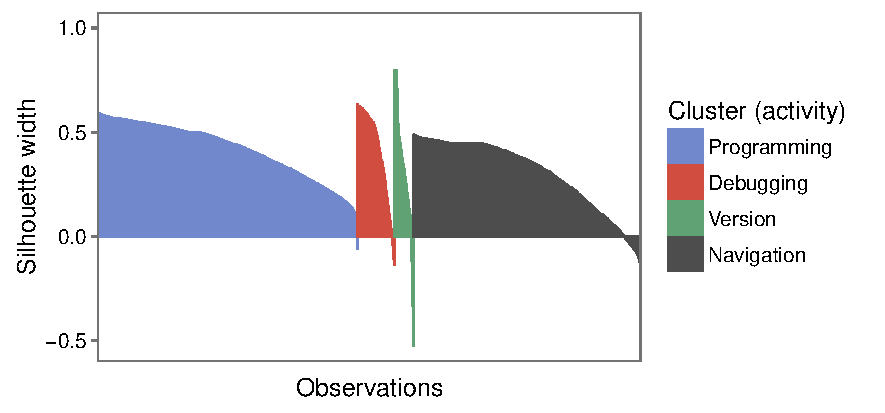
\includegraphics[width=0.7\textwidth]{Figures/UDC_silhouette_chunks}
	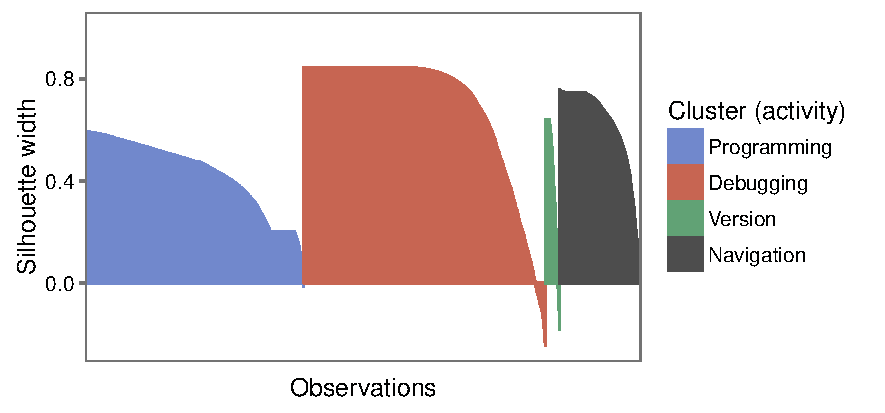
\includegraphics[width=0.7\textwidth]{Figures/ABB_silhouette_chunks}	
	\caption{Silhouette analysis of the clustering of chunks for UDC (top) and ABB (bottom).}
	\label{silhouette_chunks}
\end{figure}

In ABB the average Silhouette Average of the clusters of chunks is 0.55 and for UDC 0.38. This numbers represent a reasonable structural definition of the clusters. We can see in the Figure \ref{silhouette_chunks} the graphical representation of the silhouette of each cluster of chunks for ABB (right) and UDC (left). In average, the clusters in ABB are better defined but in both cases we can spot some observations wrongly clustered (negative values) that can also be outliers.

In the case of the clustering of sessions, we have an average silhouette of 0.35 for ABB and 0.40 for UDC, indicating also a reasonable structure but weaker than the structures in the chunks. This can be observed in the Figure \ref{silhouette_sessions}. In UDC a big number of the observations of the cluster Type C are outliers and the rest of the clusters are better defined. In ABB clusters Type A and C show good shape but the rest of the clusters have smaller averages.

\begin{figure}[!ht]
	\centering		
	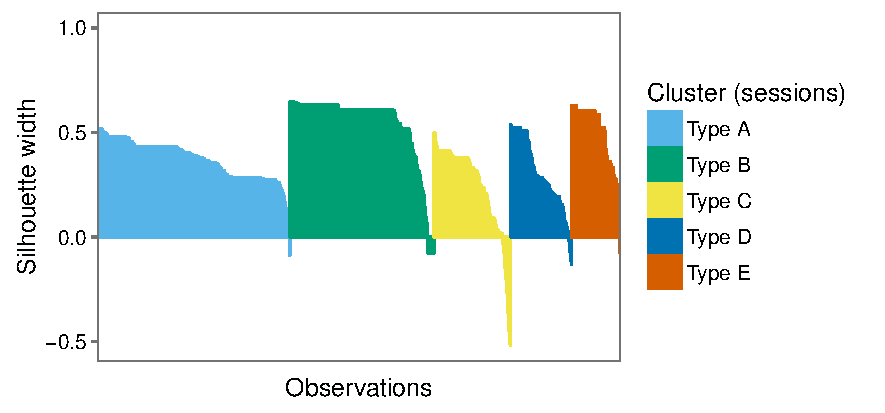
\includegraphics[width=0.7\textwidth]{Figures/UDC_silhouette_sessions}
	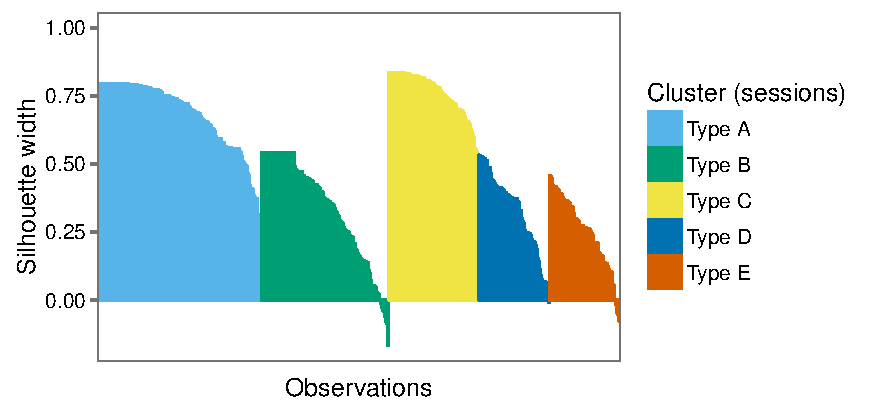
\includegraphics[width=0.7\textwidth]{Figures/ABB_silhouette_sessions}	
	\caption{Silhouette analysis of the clustering of sessions for UDC (top) and ABB (bottom).}
	\label{silhouette_sessions}
\end{figure}

Overall, we can see a clear pattern in the clustering of chunks and sessions. We believe the patterns are strong enough to support our observations and the fact there are patterns in the data. The data from ABB is stronger in this sense, probably due to the fact that it all comes from developers. In the other hand, the UDC data contains more variety of users and provokes a variety of activities and practices that are harder to cluster. 








